\chapter{MixVRTの実装}\label{cha:Implementation}
本章では、試作した\toolName の実装について説明する。
なお、本研究で用いる、\toolName の各処理部が取得または生成する画像名を、以下に定義する。
\begin{itemize}
    \item Webページの変更前画像
    \item Webページの変更後画像
    \item 高解像度にしたWebページの変更前画像
    \item 高解像度にしたWebページの変更後画像
    \item 画像比較に基づく削除箇所を赤枠で囲むことで強調表示した、Webページの変更前画像
    \item 画像比較に基づく追加箇所を緑枠で囲むことで強調表示した、Webページの変更後画像
    \item HTMLコードにおけるbody要素内の追加とstyle要素内の追加のどちらか、
          または両方の追加による影響を受けた箇所を赤枠で囲むことで強調表示した、Webページの変更前画像
    \item HTMLコードにおけるbody要素内の削除とstyle要素内の削除のどちらか、
          または両方の削除による影響を受けた箇所を緑枠で囲むことで強調表示した、Webページの変更後画像
    \item HTMLコードの変更に基づく影響箇所を色付きの枠で囲むことで強調表示した、Webページの変更前画像
    \item HTMLコードの変更に基づく影響箇所を色付きの枠で囲むことで強調表示した、Webページの変更後画像
    \item レイアウトの不具合箇所を色付きの枠で囲むことで強調表示した、Webページの変更前画像
    \item レイアウトの不具合箇所を色付きの枠で囲むことで強調表示した、Webページの変更後画像
\end{itemize}
\par
\toolName のシステム構成を、図\ref{fig:System}に示す。
\begin{figure}[tp]
    \begin{center}
        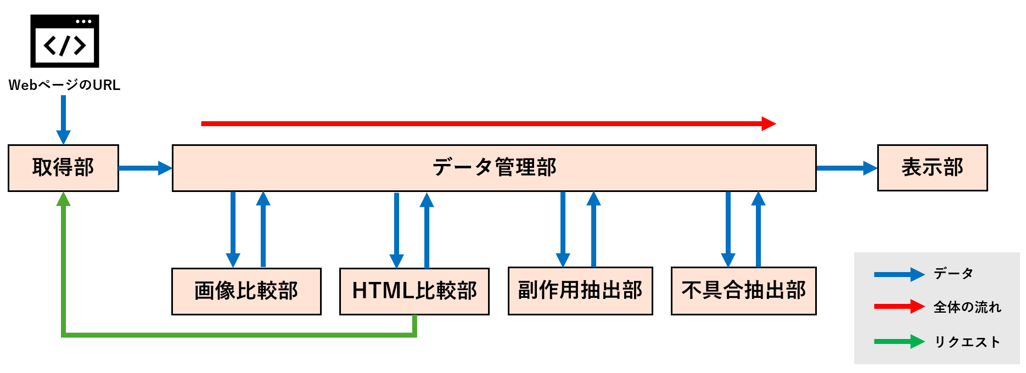
\includegraphics[width=1.0\columnwidth]{image/4_System_2.png}
        \caption{\toolName のシステム構成}
        \label{fig:System}
    \end{center}
\end{figure}
% 私の開発したツールは、まずユーザーがWebページのURLを入力します。
% このURLを受け取ると、ツールは該当するWebページから画像を取得し、
% これらの画像に対して特定の処理を行います。処理された画像は"static/images"ディレクトリに保存されます。
% そして、Flaskがローカルサーバを提供し、
% "templates"フォルダにあるHTMLコードが"static/images"ディレクトリを参照できるようになっています。
% この仕組みにより、ユーザーはローカルに立てられたFlaskサーバを通じて、
% Webページ上で生成された画像を確認することができます。
\toolName は、以下の7つの処理部から構成する。
\begin{itemize}
    \item データ管理部
    \item 取得部
    \item 画像比較部
    \item HTML比較部
    \item 副作用抽出部
    \item 不具合抽出部
    \item 表示部
          % \item 表示部
\end{itemize}
% \begin{itemize}
%     \item 取得部
%     \item 画像比較部
%           \begin{enumerate}
%               \item 差分箇所検出
%           \end{enumerate}
%     \item HTML比較部
%           \begin{enumerate}
%               \item 差分コード生成
%               \item 差分コード解析
%               \item 影響箇所強調HTMLコード生成
%           \end{enumerate}
%     \item レイアウト副作用箇所抽出部
%     \item 表示部
% \end{itemize}
以降、\toolName を構成する7つの処理部について説明する。
\par

\section{データ管理部}\label{sec:data_admin_section}
データ管理部は、システム内の各処理部間における、データの伝達を担い、他の処理部とのデータのやり取りとデータの保存を行う。
なお、本論文におけるデータとは、処理前後のWebページの画像やHTMLコードであり、
やり取りしたデータはデータ管理部が持つディレクトリに保存する。
また、取得部(\ref{sec:Web_data_get_section}節で後述)と表示部(\ref{sec:Interface_Display_Section}節で後述)のみ、データ管理部とのデータのやり取りが一方向である(図\ref{fig:System}を参照)。
% また、取得部とデータ管理部の間におけるデータのやり取りは、取得部からデータ管理部への一方向のみであり、
% データ管理部と表示部の間におけるデータのやり取りは、データ管理部から表示部への一方向のみである。
\par
データ管理部における最初のデータのやり取りは、取得部である。
取得部からデータを受け取ると、そのデータを保存する。
保存した後、データがそれ以外に存在しない場合、全体の処理を終了する。
データがそれ以外に存在する場合、
画像比較部(\ref{sec:Difference_extraction_section}節で後述)、HTML比較部(\ref{sec:Affected_area_extraction}節で後述)、
副作用抽出部(\ref{sec:Layout_subEffect_extraction_section}節で後述)、不具合抽出部(\ref{sec:Layout_bug_extraction_section}節で後述)、表示部の順に
データのやり取りを行う。
データ管理部における最後のデータのやり取りは、表示部である。
表示部に出力するデータは、\ref{subsec:MixVRT_IO}節で先述した8つのPNG形式の画像のみである。
\par
各処理部との間でやり取りしたデータを保存する各ディレクトリを、以下に示す。
\begin{itemize}
    \item base\_dirディレクトリ:\\
          取得部で取得したWebページの画像とHTMLコードを保存する。
          %   \begin{itemize}
          %       \item currentディレクトリ:\\
          %             Webページの変更前画像と変更前HTMLコードを保存する。
          %       \item latestディレクトリ:\\
          %             Webページの変更後画像と変更後HTMLコードを保存する。
          %   \end{itemize}
    \item diff\_dirディレクトリ:\\
          画像比較部、HTML比較部、副作用抽出部、不具合抽出部でやり取りしたデータを保存する。
    \item disp\_dirディレクトリ:\\
          表示部に出力するデータを保存する。
          % Webページの変更前画像と変更後画像、Webページの変更前HTMLコードと変更後HTMLコードを用いて、
\end{itemize}

% \toolName を2回実行した際の、データ管理部と各処理部とのやり取りを行ったデータを保存するディレクトリの構造を、以下に示す。

% % directory

% \begin{lstlisting}[language=, basicstyle=\ttfamily]
% .
% ├── base_dir/
% │   ├── (2回目実行時のタイムスタンプ)/
% │   │   ├── html/
% │   │   │   └── html_(2回目実行時のタイムスタンプ).html
% │   │   └── img/
% │   │       └── img_(2回目実行時のタイムスタンプ).png
% │   ├── current/ 
% │   │   ├── html/
% │   │   │   └── html_(1回目実行時のタイムスタンプ).html
% │   │   └── img/
% │   │       └── img_(1回目実行時のタイムスタンプ).png
% │   ├── initial/
% │   │   ├── html/
% │   │   │   └── html_(1回目実行時のタイムスタンプ).html
% │   │   └── img/
% │   │       └── img_(1回目実行時のタイムスタンプ).png
% │   └── latest/
% │       ├── html/
% │       │   └── html_(2回目実行時のタイムスタンプ).html
% │       └── img/
% │           └── img_(2回目実行時のタイムスタンプ).png
% └── diff_dir/
%      ├── diff_img_png/
%      │   ├── diff_af_img.png
%      │   └── diff_bf_img.png
%      ├── diff_rec_html_high_png/
%      │   ├── diff_rec_af_html.png
%      │   └── diff_rec_bf_html.png
%      ├── diff_rec_img_high_png/
%      │   ├── diff_rec_af_img.png
%      │   └── diff_rec_bf_img.png
%      ├── diff_html_txt/
%      │   └── diff_html.txt
%      ├── modified_html/
%      │   └── templates/
%      │       ├── modified_testPage_af.html
%      │       └── modified_testPage_bf.html
%      ├── modified_html_png/
%      │   ├── modified_testPage_af.png
%      │   └── modified_testPage_bf.png
%      ├── modifiled_html_high_png/
%      │   ├── modified_testPage_af_high.png
%      │   └── modified_testPage_bf_high.png
%      ├── original_high_png/
%      │   ├── img_af_high.png
%      │   └── img_bf_high.png
%      └── sub_effect_png/
%          ├── subEffect_af.png
%          └── subEffect_bf.png
% \end{lstlisting}

% \begin{itemize}
%     \item 取得部からデータ管理部
%     \item データ管理部から表示部
% \end{itemize}

% 5つの各処理部から受け付けるデータを、以下に示す。
% \begin{itemize}
%     \item 取得部:
%           \begin{itemize}
%               \item Webページの変更前画像と変更後画像
%           \end{itemize}
%     \item 画像比較部:
%           \begin{itemize}
%               \item 画像比較に基づく差分箇所を色付きの枠で囲むことで強調表示した、Webページの変更前画像と変更後画像
%               \item 上記の画像を高解像度にし、枠のみを抽出した、削除強調マスク画像と追加強調マスク画像
%           \end{itemize}
%     \item HTML比較部:
%           \begin{itemize}
%               \item HTMLコードの変更に基づく影響箇所を色付きの枠で囲むことで強調表示した、Webページの変更前画像と変更後画像
%               \item 上記の画像を高解像度にし、枠のみを抽出した、削除強調マスク画像と追加強調マスク画像
%           \end{itemize}
%     \item 副作用抽出部:
%           \begin{itemize}
%               \item レイアウトの副作用箇所を色付きの枠で囲むことで強調表示した、Webページの変更前画像と変更後画像
%           \end{itemize}
%     \item 不具合抽出部:
%           \begin{itemize}
%               \item レイアウトの不具合箇所を色付きの枠で囲むことで強調表示した、Webページの変更前画像と変更後画像
%           \end{itemize}
% \end{itemize}

% なお、\toolName の初回実行時は、取得部からWebページの画像とHTMLを受け取ると、\toolName 全体の処理を終了する。

\section{取得部}\label{sec:Web_data_get_section}
取得部は、WebページのURLを入力として受け取り、URLから取得したWebページの画像とHTMLコードをデータ管理部のbase\_dirディレクトリに出力する。
なお、HTML比較部から取得部にWebページのURLを与えて呼び出す場合があり(図\ref{fig:System}と\ref{sec:Affected_area_extraction}節を参照)、
その場合は、取得したデータをデータ管理部のdiff\_dirディレクトリに出力する。
\par
Webページの画像取得には、Selenium WebDriver(\ref{sec:Selenium_WebDriver}節を参照)を用いてWebページの画像を取得する。
なお、取得するWebページの画像は、フルページのスクリーンショット画像である。
WebページのHTMLコード取得には、Pythonライブラリの1つであるrequestsモジュール(\ref{sec:requests}節を参照)を用いて、
WebページのURLからWebページのHTMLコードを取得する。

\section{画像比較部}\label{sec:Difference_extraction_section}
画像比較部は、データ管理部のbase\_dirディレクトリからWebページの変更前画像と変更後画像を受け取り、
画像比較に基づく差分箇所を色付きの枠で囲むことで強調表示したWebページの変更前画像と変更後画像を生成する。
また、それらの画像から枠のみを残してそれ以外の部分を黒くすることで、差分箇所を囲む色付きの枠のみを抽出した、「差分箇所赤枠強調マスク画像」と「差分箇所緑枠強調マスク画像」も生成する。
生成した画像は、データ管理部のbase\_dirディレクトリに出力する。
\par
画像比較部の処理の流れを、以下に示す。
\begin{enumerate}
    \item 高解像度画像生成処理
    \item 適応的二値化処理
    \item 差分検出処理
    \item 膨張処理
    \item 輪郭検出処理
    \item 枠描画処理
\end{enumerate}
以降、画像比較部の各処理について説明する。

\subsection{高解像度画像生成処理}\label{subsec:Generate_high_images}
高解像度画像生成処理は、Webページの変更前画像と変更後画像をそれぞれ高解像度画像にした、「変更前高解像度画像」と「変更後高解像度画像」を生成する。
この処理は、輪郭検出処理(\ref{subsec:contour_detection_processing}節で後述)の精度を向上するために必要である。
なお、生成した高解像度画像は他の処理部で使用するため、「変更前高解像度画像」と「変更後高解像度画像」をデータ管理部のbase\_dirディレクトリに出力する。
\par
高解像度画像を生成する流れを、以下に示す。なお、リサイズに使用するリサンプリングフィルタには、LANCZOSフィルタ(\ref{sec:pillow}節を参照)を用いる。
\begin{enumerate}
    \item PillowのImage.open関数(\ref{sec:pillow}節を参照)を用いて、Webページの画像パスから画像を読み込む。
    \item 画像の幅と高さを取得する。
    \item 画像の拡大率を設定する。本研究では、$2$とする。
    \item 画像のサイズ変更時に使用するリサンプリングフィルタを設定する。本研究では、PillowのImage.LANCZOSフィルタ(\ref{sec:pillow}節を参照)を用いる。
    \item Webページの画像を、画像の幅と高さにそれぞれ画像の拡大率を掛けたサイズの高解像度画像にリサイズする。
\end{enumerate}

\subsection{適応的二値化処理}\label{subsec:Adaptive_Binarisation}
適応的二値化処理は、「変更前高解像度画像」と「変更後高解像度画像」のそれぞれに対して、適応的二値化を行う。
この処理により、画像の一部が明るく、他の部分が暗い場合においても、全体として均一な二値化画像を生成できるため、
輪郭検出処理(\ref{subsec:contour_detection_processing}節で後述)の精度向上につながる。
処理の結果として、適応的二値化処理を行った、「変更前高解像度二値化画像」と「変更後高解像度二値化画像」を生成する。
\par
「変更前高解像度画像」と「変更後高解像度画像」に対して、それぞれ適応的二値化を行う流れを、以下に示す。
\begin{enumerate}
    \item OpenCVのimread関数(\ref{sec:opencv}節を参照)を用いて、画像を読み込む。
    \item OpenCVのcvtColor関数(\ref{sec:opencv}節を参照)を用いて、画像をグレースケール化する。
    \item OpenCVのadaptiveThreshold関数(\ref{sec:opencv}節を参照)を用いて、画像の適応的二値化を行う。
\end{enumerate}


\subsection{差分検出処理}\label{subsec:difference_detection_process}
差分検出処理は、subtract関数\ref{sec:opencv}を用いて、「変更前高解像度二値化画像」と「変更後高解像度二値化画像」に対して、差分検出を行う。
処理の結果として、Webページの変更前画像から削除された箇所と、Webページの変更後画像に追加された箇所をそれぞれ白い部分として可視化した、
「削除箇所二値化画像」と「追加箇所二値化画像」を生成する。

\subsection{膨張処理}\label{subsec:dilation}
% (\ref{sec:dilation}節を参照)
膨張処理は、「削除箇所二値化画像」と「追加箇所二値化画像」のそれぞれの白い部分の形状とサイズを強調する。
この処理により、削除箇所と追加箇所の輪郭検出処理(\ref{subsec:contour_detection_processing}節で後述)を高める。
処理の結果として、膨張処理を行った、「削除箇所強調二値化画像」と「追加箇所強調二値化画像」を生成する。
\par
「削除箇所二値化画像」と「追加箇所二値化画像」に対して、膨張処理を適用する流れを、以下に示す。
\begin{enumerate}
    \item 特定の形状とサイズを持つカーネルを設定する。本研究では、5x5ピクセルの正方形カーネルを採用する。
    \item 設定したカーネルを用いて、膨張処理を適用する。適用後、画像内の削除箇所または追加箇所が拡大する。
    \item 2の膨張処理を複数回適用する。本研究では、膨張処理を6回繰り返すことで削除箇所または追加箇所を強調する。
\end{enumerate}

\subsection{輪郭検出処理}\label{subsec:contour_detection_processing}
輪郭検出処理は、OpenCVのfindContours関数(\ref{sec:opencv}節を参照)を用いて、「削除箇所強調二値化画像」と「追加箇所強調二値化画像」に対して、
削除箇所の輪郭と追加箇所の輪郭をそれぞれ検出する。
この処理の結果として、削除箇所の輪郭リストと追加箇所の輪郭リストを取得する。

\subsection{枠描画処理}\label{subsec:Bounding box drawing process}
枠描画処理は、Webページの変更前画像と変更後画像に対して、
輪郭検出処理(\ref{subsec:contour_detection_processing}節を参照)で取得した輪郭リストを用いて、
画像比較に基づく差分箇所を色付きの枠で囲むことで強調表示したWebページの変更前画像と変更後画像を生成する。
また、それらの画像から枠のみを残してそれ以外の部分を黒くすることで、差分箇所を囲む色付きの枠のみを抽出した、
「差分箇所赤枠強調マスク画像」と「差分箇所緑枠強調マスク画像」を生成する。
\par
枠描画処理の流れを、以下に示す。
\begin{enumerate}
    \item cv2.boundingRect関数(\ref{sec:opencv}節を参照)を用いて、輪郭リストの各要素である輪郭データから、輪郭を囲む矩形の座標と幅、高さを取得する。
    \item 取得した矩形情報を引数に指定したcv2.rectangle関数(\ref{sec:opencv}節を参照)を用いて、Webページの変更前画像上に赤枠、Webページの変更後画像上に緑枠を描画する。
    \item Webページの変更前画像と変更後画像のそれぞれと同じサイズの黒画像を生成する。
    \item 生成した2つの黒画像に対して、一方の黒画像には赤枠を、もう一方の黒画像には緑枠を描画する。
\end{enumerate}

%%%% HTML比較 %%%%
\section{HTML比較部}\label{sec:Affected_area_extraction}
HTML比較部は、取得部からWebページの変更前HTMLコードと変更後HTMLコードを受け取り、
HTMLコードの変更に基づく影響箇所を色付きの枠で囲むことで強調表示した、Webページの変更前画像と変更後画像を生成する。
また、それらの画像から枠のみを残してそれ以外の部分を黒くすることで、影響箇所を囲む色付きの枠のみを抽出した、変更前画像と変更後画像も生成する。
なお、影響箇所を囲む色付きの枠のみを抽出した、変更前画像と変更後画像に関しては、レイアウトの副作用抽出部に処理画像として出力する。
\par
HTML比較部の処理の流れを、以下に示す。
\begin{enumerate}
    \item 差分コード生成処理
    \item 差分コード解析処理
    \item 影響箇所強調HTMLコード生成処理
    \item 枠抽出処理
\end{enumerate}
以降、HTML比較部の各処理について説明する。

\subsection{差分コード生成処理}\label{subsec:diff_file_generate}
差分コード生成処理は、Webページの変更前HTMLコードと変更後HTMLコードを行ごとに比較して、差分コードをtxt形式として生成する。
なお、生成した差分コードは、コードの追加行には"+", 削除行には"-", 変更前後のHTMLコードにどちらにも存在しない行には"?"が先頭に自動で付き、"?"を除いた差分コードを解析対象とする。
\par
差分コードを生成する処理を、以下に示す。
\begin{enumerate}
    \item 変更前HTMLコードと変更後HTMLコードをそれぞれHTMLデータとして読み込む。
    \item difflibモジュール(\ref{sec:difflib}節を参照)を使用して、2つのHTMLデータ間を行ごとに比較する。
    \item 差分コードをtxt形式で保存する
\end{enumerate}

\subsection{差分コード解析処理}\label{subsec:diff_file_analyze}
差分コード解析処理は、差分コード生成処理から差分コードを受け取り、差分コードからbody要素内の変更箇所とstyle要素内の変更箇所を見つける。

\subsection{枠付きHTMLコード生成処理}\label{subsec:modified_html_generate}
枠付きHTMLコード生成処理は、差分コード解析処理から変更箇所を受け取り、変更箇所に色付きの枠をつけるcssクラスを追加したHTMLコードを生成する。
なお、変更箇所に色付きの枠をつけるcssクラスを追加したHTMLコードを、枠付きHTMLコードと定義する。

\subsection{枠抽出処理}\label{subsec:frame_extraction}
枠抽出処理は、Webページの変更前画像と枠付きを行ったWebページの変更前画像を比較し、赤枠のみを抽出した画像を生成する。
また、Webページの変更後画像と枠付きを行ったWebページの変更後画像を比較し、緑枠のみを抽出した画像を生成する。
生成した画像は、レイアウトの副作用抽出部に出力する。
\par
枠抽出処理の流れを、以下に示す。
\begin{enumerate}
    \item 枠付きHTMLコードをローカルサーバ上でWebページとして公開する
    \item 取得部を用いて、枠付きHTMLをもとにしたWebページの画像を取得する
    \item Webページの変更前画像と枠付きを行ったWebページの変更前画像を比較し、赤枠のみを抽出した変更前画像を生成する
    \item Webページの変更後画像と枠付きを行ったWebページの変更後画像を比較し、緑枠のみを抽出した画像を生成する
\end{enumerate}

% \section{影響箇所検出部}\label{sec:Affected_area_extraction}
% HTMLコードの変更に基づく影響箇所抽出部は、Webページ情報取得部で取得した変更前後のWebページのHTMLコードを用いて影響箇所を特定する。
% 概要としては、差分コードを生成し、差分コードから枠付き処理を行った変更前後のHTMLコードを生成した後、そのHTMLコードをFlaskのテンプレートエンジンを用いてWebページを表示し、Webページ情報取得部によってそのWebページの画像を取得する。
% 元のWebページ画像と枠付き処理をしたWebページ画像を比較して枠のみを抽出する。
% 具体的には、まず、Pythonライブラリの一つであるdifflibモジュールを用いて、変更前後のHTMLコードから差分コードを生成する。
% 生成した差分コードは、コードの追加行には"+", 削除行には"-", 変更前後のHTMLコードにどちらにも存在しない行には"?"が先頭に付き、"?"を除いた差分コードを解析対象とする。
% 差分コードは、bodyタグ内とstyleタグ内を対象とする。
% もし、bodyタグ内で先頭に"+"や"-"があれば、コードの追加や削除、変更があったとして、その箇所に枠付き処理を行うCSSクラスを追加し、先頭の"+"か"-"を削除する。
% styleタグ内の場合は、CSSクラスのセレクタ名のみの変更やスタイルのみの変更、またはその両方の変更があったCSSクラスを対象として、そのCSSクラスに対して枠付きを行うスタイルを適用する。
% この場合においても、解析した行の先頭に"+", "-"があれば削除する。
% 差分コードから枠付き処理を行った変更前後のHTMLコードを生成した後は、そのHTMLコードをFlaskのテンプレートエンジンを用いてWebページとして表示し、そのWebページの画像を取得する。
% そして、元のWebページ画像と枠付き処理をしたWebページ画像を比較して枠のみを抽出する。
\section{レイアウトの副作用検出部}\label{sec:Layout_subEffect_extraction_section}
レイアウトの副作用抽出部は、画像比較に基づく差分箇所とHTMLコードの変更に基づく影響箇所を用いて、レイアウトの副作用箇所を抽出する。
具体的には、差分箇所を囲む枠と影響箇所を囲む枠同士を比較する。比較の仕方は、枠の重なり度合を判定する。
まず、枠が重なっているかどうかを判定する。次に、枠が重なっている場合に、重なり部分が小さい方の枠の面積の6割以上であれば枠が一致すると判定する。
最終的に、一致しない枠のみを抽出し、一致しない赤枠をWebページの変更前画像に、一致しない緑枠をWebページの変更後画像に描画し、保存する。

\section{レイアウトの不具合検出部}\label{sec:Layout_bug_extraction_section}
レイアウトの不具合抽出部は、レイアウトの副作用抽出部から抽出したレイアウトの副作用箇所から、レイアウトの不具合箇所を抽出する。
具体的には、\ref{sec:Layout_subEffect_extraction_section}節で抽出したレイアウトの副作用箇所を囲んだ各赤枠内の領域と、レイアウトの副作用箇所を囲んだ各緑枠内の領域を比較する。
その後、赤枠内の領域と緑枠内の領域をabsdiff関数(\ref{sec:Layout_subEffect_extraction_section}節を参照)で絶対差分を計算して類似度を求める。
類似度が9割を超えれば、レイアウトの不具合は無いと判定し、比較した赤枠と緑枠を除外する。
上記の処理によって、類似度が9割未満であった赤枠と緑枠を抽出することができ、それらはレイアウトの不具合として、Webページの変更前画像と変更後画像をする。


\section{表示部}\label{sec:Interface_Display_Section}
表示部は、
\ref{sec:Web_data_get_section}節~\ref{sec:Layout_subEffect_extraction_section}節で取得・生成した画像(枠強調マスク画像を除く)を保管し、
Webベースのinterfaceユーザを用いて表示する。
MixVRTの実行コマンド初回実行時は、\ref{sec:Web_data_get_section}節で取得したWebページの画像を保管する。
MixVRTの実行コマンド2回目以降実行時は、初回実行時に取得する画像に加えて、\ref{sec:Difference_extraction_section}節で取得した画像、
\ref{sec:Affected_area_extraction}節で生成した画像、\ref{sec:Layout_subEffect_extraction_section}節で生成した画像を保管する。



% \section{画像とHTMLコード取得部}\label{sec:area_detection_part}

% \subsection{Seleniumによる画像取得}\label{subsec:rect_detection}

% \subsection{requestsによるHTMLコード取得}\label{subsec:underline_detection}


% \section{差分抽出部}\label{sec:OCR_part}

% \subsection{画像比較による差分抽出}\label{subsec:char_extraction}

% \subsection{HTMLの変更による影響箇所抽出}\label{subsec:bbox_coords_obtainment}

% \subsection{画像とHTMLコードに基づくレイアウトの副作用抽出}\label{subsec:bbox_obtainment}


% \section{差分表示部}\label{sec:label_link_part}